\chapter{Introduction}
\label{Chapter1}
\section{Motivation}

Our current approach discards edge saliency information (the Structured edge~\cite{DollarICCV13edges} output - probability of boundary values) and instead relies only on the structured information contained in the trained Structured forest.

\section{Terminology}
\subsection{Edge Detection - Edge, Edge Map, Probability of Boundary}
%- application in tasks such as object detection/recognition, structure from motion, segmentation and tracking
%- general consensus in the community that edge detection is somewhat ill defined in that it is not quiteclear what defines a correct output \cite{martin2004learning}

Image edge detection deals with the problem of finding pixels which belong to object boundaries within a digital image. The pixels belonging to object boundaries in an image are often locations where a sharp change of image brightness occurs. Those locations of image intensity discontinuities, typically grouped together, are called image edges.

We will call an edge map a binary image depicting edges locations. The pixels belonging to an edge are set to 1. The rest of the pixels are not part of an edge. They have a value of 0. Therefore, for a given pixel location $(x,y)$, the corresponding edge map value is $em_{x,y} \in \{0,1\}$

To allow to express a level of (un)certainty as to the presence of an edge in an image, we employ a probabilistic means. We define a real-valued image called a Probability of boundary (Pb) (see Figure~\ref{fig:edge_detection}\subref{fig:subfigure2}). The notion of probability of a location being an edge point was first introduced in \cite{martin2004learning}. It has ever since been used as an output to many edge detection algorithms \cite{Maire2008using}.

\begin{figure}[ht!]
 \centering
 \subfigure[Input image]{%
 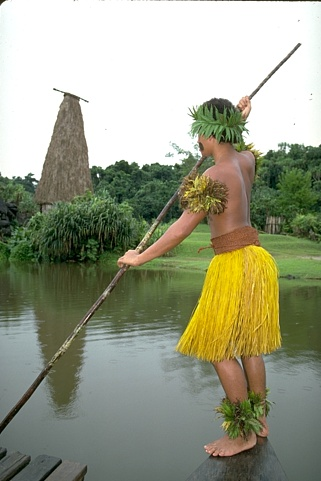
\includegraphics[width=0.3\textwidth]{images/examples/hawaii/arbelaez2011-035.png}
\label{fig:subfigure1}}
 \subfigure[Edge map]{%
 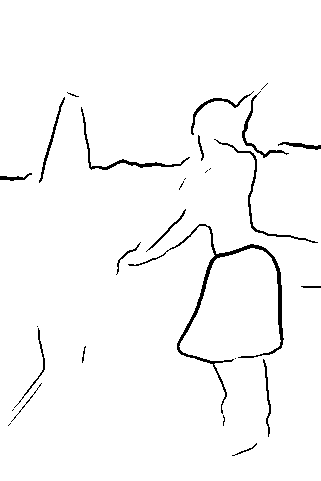
\includegraphics[width=0.3\textwidth]{images/examples/hawaii/edge_map_arbelaez2011-039.png}
\label{fig:subfigure2}}
\subfigure[Probability of boundary]{%
 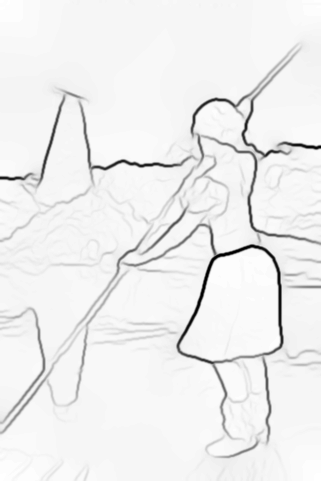
\includegraphics[width=0.3\textwidth]{images/examples/hawaii/Pb_arbelaez2011-039.png}
\label{fig:subfigure3}}
% \quad
% \qquad
 \caption[Caption that doesn't show?]{{\bf Edge detection} (courtesy of~\cite{Arbelaez11}). Note that for ease of view %illustration
 , the negative of the probability is shown, \ie the darker the pixel, the higher the probability of an edge.}
\label{fig:edge_detection}
\end{figure}

\subsection{Image Segmentation - Contour, Segmentation, Region Boundary, Hierarchical Segmentation}
\section{Related Work}
% \subsubsection*{Edge Detection}
\subsection{From Edges to Contours}
\subsubsection{Edge Detection}
Early edge detection approaches solely rely on local cues. Low-level detectors define edges as sharp discontinuities in image brightness. First results were achieved using digital image processing techniques. The Roberts cross~\cite{roberts1963machine}, Sobel filter~\cite{sobel19683x3}, and Prewitt operator~\cite{prewitt1970object} all are discrete differentiation operators. % can say 'differential operator'
They view an images as a 2-dimensional signal which they convolve with pre-defined filters with local support. In the same line of work is the Marr-Hildreth algorithm~\cite{marr1980theory}, which finds zero-crossings of the Laplacian of the image intensity. Later still, the Canny detector~\cite{canny1986computational} shows better-quality edges. It searches for peak gradient magnitude in the image intensity. It adds some improvements, like non-maximum suppression (also known as ``edge thinning''), which improves edge localisation. A practically relevant extensions of it is the Canny-Deriche detector~\cite{deriche1987using}, which addresses the filter implementation.

More higher-level detectors incorporate colour and texture~\cite{rubner1996coalescing,will2000learning} information, as well as multiple scales and orientations.

Globalisation-based methods.

Recent approaches are interested in high quality edge detection. They therefore rely on learning to incorporate context and object knowledge. They address more challenging scenarios which arise in natural images. As Martin \etal argue in \cite{martin2004learning}, those methods solve the so-called ``boundary detection'' problem. A boundary delineates the pixels that belong to one object, material, or surface from those that belong to another. One possible approach to boundary detection would be to use edges as low-level cues to judge for the presence of object boundaries (a bottom-up approach). Another solution is to go top-down and use higher-level object knowledge to infer the object boundaries.

In such more challenging situations a \textit{general} edge detector would not be adequate, since the desired output is application-specific.


\subsubsection{Image Segmentation}
\subsection{State-of-the-Art Review}
\section{Goal}
% a more principled approach to boundary-guided image segmentation. % analysis?
\section{Outline}
The rest of this work is structured as follows:

% \begin{itemize}
% \item Chapter~\ref{SpectRelax} starts the thesis with a brief introduction to balanced graph cuts and spectral relaxation techniques.
% Section~\ref{sec:ch2_clgrpart} shows that clustering can be seen as a graph partitioning problem. The minimum cut approach often yields useless results where clusters are highly unbalanced, hence
% the balanced graph cut criteria are described in Section~\ref{sec:ch2_balgrcut}.  To solve the NP-hard balanced graph cut problem
% the relaxation methods are applied. Section~\ref{sec:ch2_spectclus} presents the standard spectral clustering approach, which is known to be loose.
% The tight relaxation, called 1-spectral clustering, is described in Section~\ref{sec:ch2_1spectclus}. 
% Section~\ref{ch2:disc} concludes the chapter and discusses the relevance of proposed methods to video segmentation.
% \item Chapter~\ref{chapter3} gives an overview of the video segmentation framework and provides the analysis of low-level features.
% Section~\ref{sec:ch3_framework} introduces the proposed video segmentation model, which employs a two-step approach:
% a graph is constructed on pre-computed superpixels and then a spectral clustering technique is applied. 
% %In graph-based algorithms, in order to produce high-quality segmentation results powerful superpixel similarity measures must be defined.
% Section~\ref{sec:ch3_affinities} gives a description of the graph affinities used in this work.
% To evaluate video segmentation performance and analyze the features of the proposed model we chose the Berkeley motion segmentation dataset, which is presented in Section~\ref{sec:ch3_dataset}.  
% The examination of the quality of the low-level video features is reported in Section~\ref{sec:ch3_aff} and the results are discussed in Section~\ref{ch3:disc}.
% \item Chapter~\ref{Chapter4} provides an experimental comparison of spectral relaxations and analyzes the effects of different balanced graph cuts applied to video segmentation. 
% We start with a brief recap of the main theoretical aspects of 1-norm and 2-norm relaxations in Section~\ref{ch4:recap}.
% Section~\ref{ch4:bench} presents the evaluation benchmark for video segmentation.
% Section~\ref{sec:ch4_1sc_vs_sc} shows the comparison of the performance of spectral clustering and 1-spectral clustering with different balanced graph cut objectives in the task of video segmentation. 
% In order to explore further the balanced cut criteria and the quality of the solutions obtained from the relaxation techniques, we tried to find a better partition by a trivial greedy search optimizing different balanced graph cut functions and see if the ground truth corresponds
% with the minimum cut criterion. The results of the experiments are reported in Section~\ref{sec:ch4_GTexp}.
% Section~\ref{ch4:disc} gives the discussion of the obtained results.
% \item In Chapter~\ref{Chapter5} a methodology for discriminative learning of must-link constraints and their incorporation in the video segmentation framework are proposed.
% Section~\ref{sec:ch5_cosc} shows a way of integrating prior information in the form of must-link constraints into spectral clustering while preserving all the
% balanced graph cuts.
% Section~\ref{sec:llf} presents evaluation of the low-level features as must-link constraints and the connections in the graph based on the ground truth.
% In Section~\ref{sec:ch4_ML} we propose to learn must-links with Random Forest from the affinities.
% We show that even a naive learning approach on the restricted feature space improves video segmentation performance for both relaxations: spectral clustering and 1 spectral clustering. 
% The proposed model is compared to state-of-the-art methods.
% Section~\ref{ch5:disc} discusses the achieved results.
% \item Chapter~\ref{Chapter6} concludes the thesis summarizing all the results of our work and proposing directions for possible improvements.
% \end{itemize}
